\addcontentsline{toc}{section}{Part IV - State estimation}
\section*{Part IV - State estimation}
\addcontentsline{toc}{subsection}{5.4.1 Problem 1}
\subsection*{5.4.1 Problem 1}
We now have that
\begin{align*}
x &= 
\begin{bmatrix}
    \tilde{p}\\
    \dot{\tilde{p}}\\
    \tilde{e}\\
    \dot{\tilde{e}}\\
    \tilde{\lambda}\\
    \dot{\tilde{\lambda}}
\end{bmatrix},\; u =
\begin{bmatrix}
    \tilde{V_s}\\
    \tilde{V_d}
\end{bmatrix}\; \text{and}\;
y = 
\begin{bmatrix}
    \tilde{p}\\
    \tilde{e}\\
    \tilde{\lambda}
\end{bmatrix}
\intertext{Substituting for the state-space formula we get that}
\dot{x} &= 
\begin{bmatrix}
    \dot{\tilde{p}}\\
    \ddot{\tilde{p}}\\
    \dot{\tilde{e}}\\
    \ddot{\tilde{e}}\\
    \dot{\tilde{\lambda}}\\
    \ddot{\tilde{\lambda}}
\end{bmatrix} = 
A\begin{bmatrix}
    \tilde{p}\\
    \dot{\tilde{p}}\\
    \tilde{e}\\
    \dot{\tilde{e}}\\
    \tilde{\lambda}\\
    \dot{\tilde{\lambda}}
\end{bmatrix} + 
B \begin{bmatrix}
    \tilde{V_s}\\
    \tilde{V_d}
\end{bmatrix}
\end{align*}
\begin{align*}
\begin{bmatrix}
    \dot{\tilde{p}}\\
    \ddot{\tilde{p}}\\
    \dot{\tilde{e}}\\
    \ddot{\tilde{e}}\\
    \dot{\tilde{\lambda}}\\
    \ddot{\tilde{\lambda}}
\end{bmatrix} &= 
\begin{bmatrix}
    0 & 1 & 0 & 0 & 0 & 0\\
    0 & 0 & 0 & 0 & 0 & 0\\
    0 & 0 & 0 & 1 & 0 & 0\\
    0 & 0 & 0 & 0 & 0 & 0\\
    0 & 0 & 0 & 0 & 0 & 1\\
    K_3 & 0 & 0 & 0 & 0 & 0\\
\end{bmatrix}
\begin{bmatrix}
    \tilde{p}\\
    \dot{\tilde{p}}\\
    \tilde{e}\\
    \dot{\tilde{e}}\\
    \tilde{\lambda}\\
    \dot{\tilde{\lambda}}
\end{bmatrix} + 
\begin{bmatrix}
    0 & 0\\
    0 & K_1\\
    0 & 0\\
    K_2 & 0\\
    0 & 0\\
    0 & 0\\
\end{bmatrix}
\begin{bmatrix}
    \tilde{V_s}\\
    \tilde{V_d}\\
\end{bmatrix}
\\
y &= Cx = 
\begin{bmatrix}
    1 & 0 & 0 & 0 & 0 & 0\\
    0 & 0 & 1 & 0 & 0 & 0\\
    0 & 0 & 0 & 0 & 1 & 0
\end{bmatrix}
\begin{bmatrix}
    \tilde{p}\\
    \dot{\tilde{p}}\\
    \tilde{e}\\
    \dot{\tilde{e}}\\
    \tilde{\lambda}\\
    \dot{\tilde{\lambda}}
\end{bmatrix}
\end{align*}



\newpage
\addcontentsline{toc}{subsection}{5.4.2 Problem 2}
\subsection*{5.4.2 Problem 2}
To examine the observability of the system, we need to calculate wether or not the observability matrix has full rank or not. The observability matrix $\mathcal{O}$ is given by

\begin{align*}
\mathcal{O} = \begin{bmatrix}
C\\
CA\\
CA^2\\
CA^3\\
CA^4\\
CA^5
\end{bmatrix}
=
\begin{bmatrix}
1 & 0 & 0 & 0 & 0 & 0\\
0 & 0 & 1 & 0 & 0 & 0\\
0 & 0 & 0 & 0 & 1 & 0\\
0 & 1 & 0 & 0 & 0 & 0\\
0 & 0 & 0 & 1 & 0 & 0\\
0 & 0 & 0 & 0 & 0 & 1\\
0 & 0 & 0 & 0 & 0 & 0\\
0 & 0 & 0 & 0 & 0 & 0\\
K_3 & 0 & 0 & 0 & 0 & 0\\
0 & 0 & 0 & 0 & 0 & 0\\
0 & 0 & 0 & 0 & 0 & 0\\
0 & K_3 & 0 & 0 & 0 & 0\\
0 & 0 & 0 & 0 & 0 & 0\\
0 & 0 & 0 & 0 & 0 & 0\\
0 & 0 & 0 & 0 & 0 & 0\\
0 & 0 & 0 & 0 & 0 & 0\\
0 & 0 & 0 & 0 & 0 & 0\\
0 & 0 & 0 & 0 & 0 & 0
\end{bmatrix}
\end{align*}
As we can see, $\mathcal{O}$ has full rank, and the system is observable. Next, a linear observer for the system is created
\begin{align*}
\dot{\hat{x}} = A\hat{x} + Bu + L(y - C\hat{x})
\end{align*}
the observer error $e$ is given by
\begin{align*}
e =  x -\hat{x}
\end{align*}
we derive and find that the error estimate satisfy
\begin{align*}
\dot{e}     &= \dot{x} - \dot{\hat{x}}\\
            &= Ax+Bu-A\hat{x}-Bu-L(y-C\hat{x}-Du)\\
            &= Ax - A\hat{x} -Ly + LC\hat{x} + LDu\\
            &= A(x -\hat{x})- L(Cx + Du) + LC\hat{x} + LDu\\
            &= Ae - LC(x - \hat{x})\\
            &= (A - LC)e
\end{align*}
\begin{comment}
When {A,C} is observable an appropriate observer gain L can be chosen by assigning the eigenvalues of A − LC to achieve a certain convergence rate for e.
\end{comment}

The system then equals
\begin{align*}
\begin{bmatrix}
    \dot{\hat{x}}\\
    \dot{e}
\end{bmatrix}\ = \
\begin{bmatrix}
    A-BK     &   BK\\
    0        &   A-LC
\end{bmatrix}
\begin{bmatrix}
    x\\
    e
\end{bmatrix}\ + \
\begin{bmatrix}
    BP\\
    0
\end{bmatrix}r
\end{align*}

We are able to choose the $L$ independentaly from the already choosen $K$ because of the principle of seperation. \\
\begin{figure}[H]
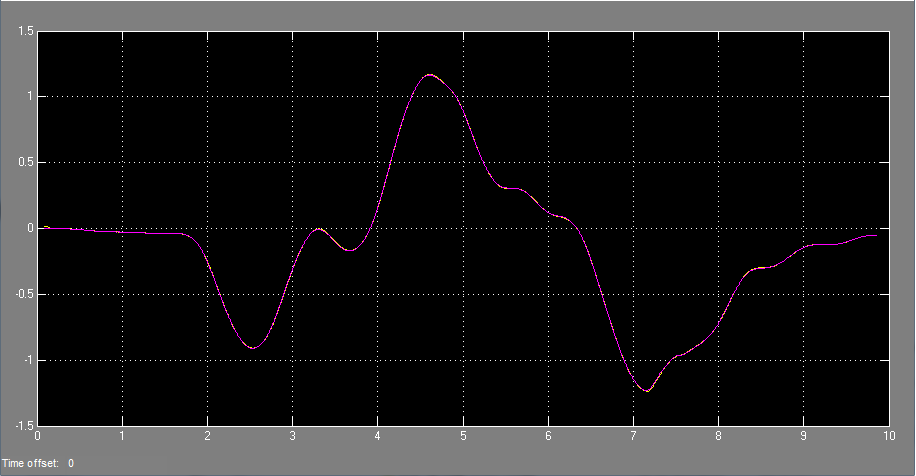
\includegraphics[width=0.9\textwidth,height=0.1\textheight]{Pitch.png}\\
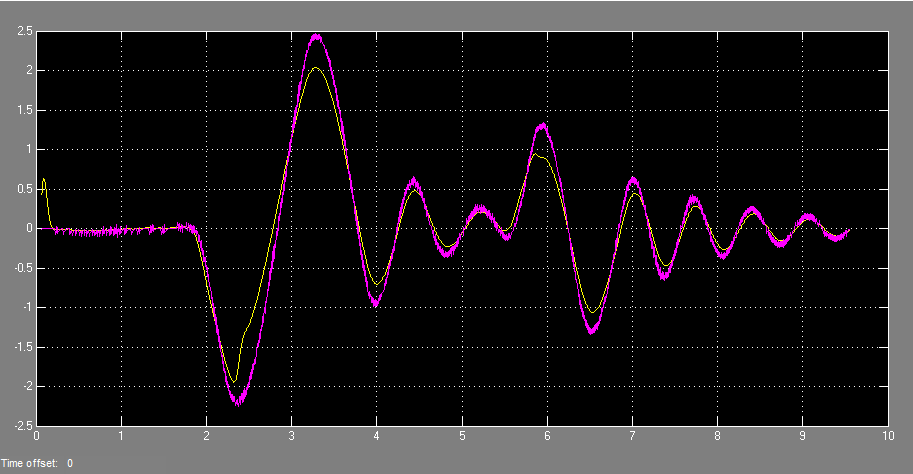
\includegraphics[width=0.9\textwidth,height=0.1\textheight]{Pitch_Rate.png}\\
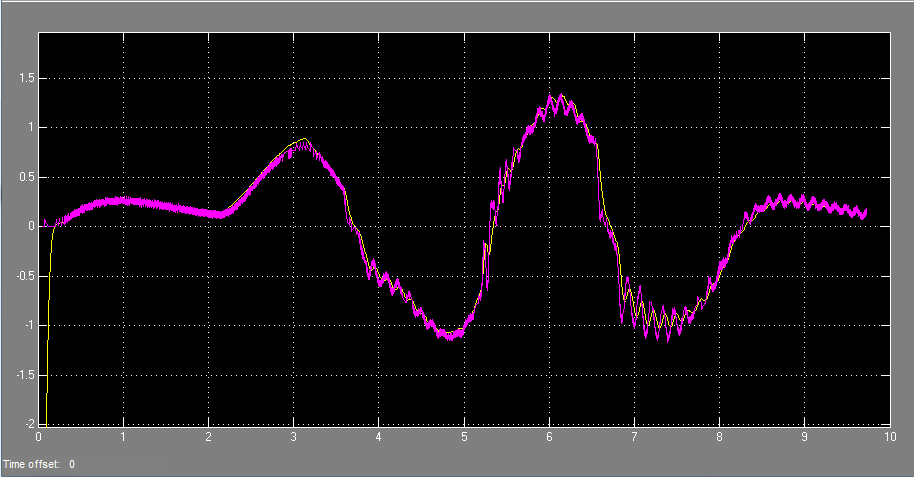
\includegraphics[width=0.9\textwidth,height=0.1\textheight]{Elevation_Rate.png}\\
\caption{Estimated states (purple) vs. measured states (yellow) for the 3-input observer, with P controller}
\label{fig:my_label}
\end{figure}

\begin{figure}[H]
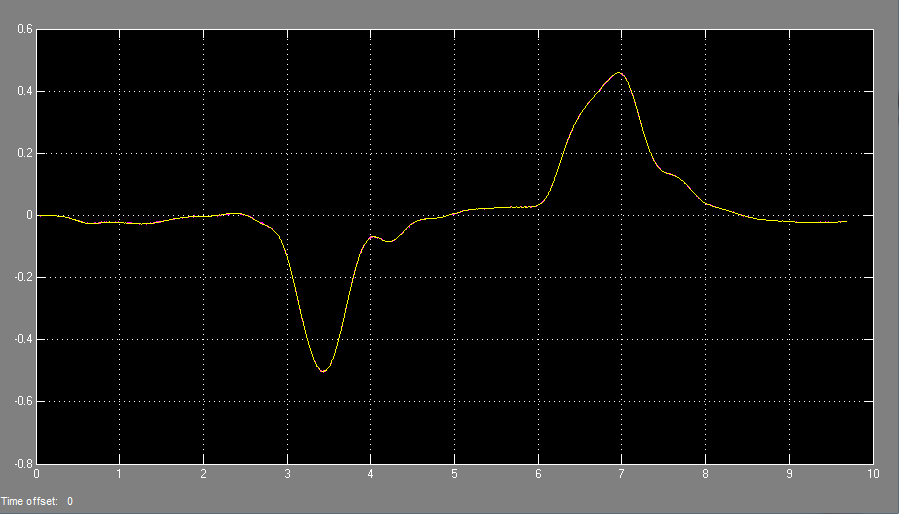
\includegraphics[width=0.9\textwidth,height=0.1\textheight]{PI_Pitch.png}\\
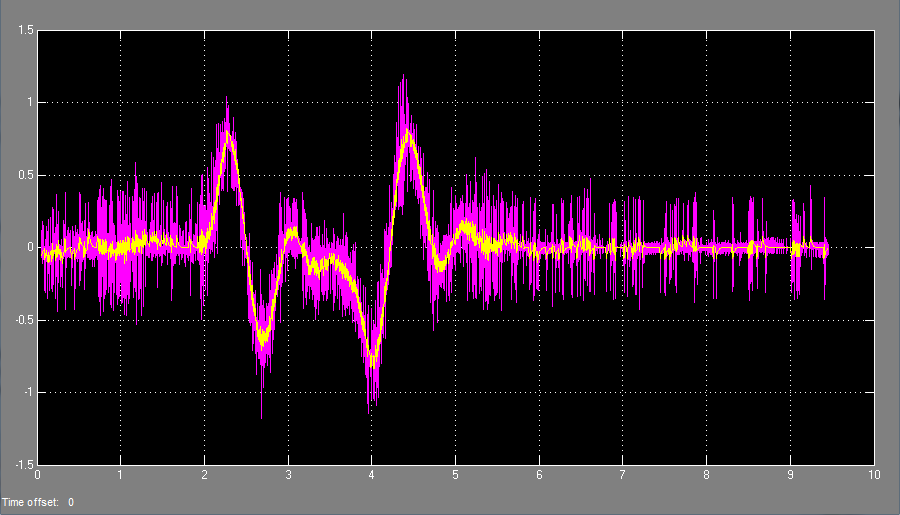
\includegraphics[width=0.9\textwidth,height=0.1\textheight]{PI_Pitch_Rate.png}\\
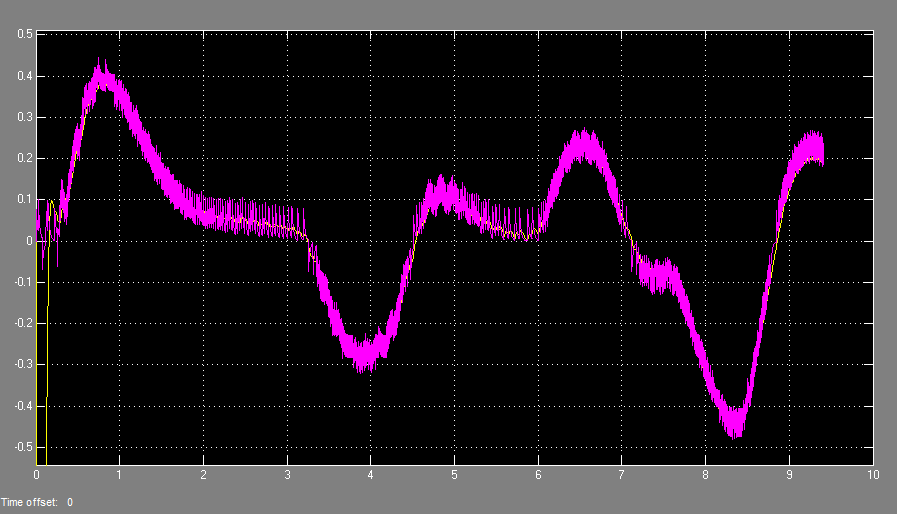
\includegraphics[width=0.9\textwidth,height=0.1\textheight]{PI_Elevation_Rate.png}
\caption{Estimated states (purple) vs. measured states (yellow) for the 3-input observer, with PI controller}
\label{fig:my_label2}
\end{figure}

The estimated states seem to converge to the true states while significantly filtering out measurement noise for the pitch and pitch rate. The necessary speed of the observer, i.e the radius of the pole placements, was around 100 times greater than the closed loop controllers. While the speed of the observer was seen to greatly affect the quality of the estimation and thus the response of the helicopter, variation of the angular spread in the pole placements did not generate any great effects.

\newpage
\addcontentsline{toc}{subsection}{5.4.3 Problem 3}
\subsection*{5.4.3 Problem 3}
If $\tilde{e}$ and $\tilde{\lambda}$ are measured, $C$ is given by
\begin{align*}
C =
\begin{bmatrix}
    0 & 0 & 1 & 0 & 0 & 0\\
    0 & 0 & 0 & 0 & 1 & 0
\end{bmatrix}
\end{align*}
Giving the observability matrix
\begin{align*}
\mathcal{O} =
\begin{bmatrix}
    0 & 0 & 1 & 0 & 0 & 0\\
    0 & 0 & 0 & 0 & 1 & 0\\
    0 & 0 & 0 & 1 & 0 & 0\\
    0 & 0 & 0 & 0 & 0 & 1\\
    K_3 & 0 & 0 & 0 & 0 & 0\\
    0 & K_3 & 0 & 0 & 0 & 0\\
    0 & 0 & 0 & 0 & 0 & 0\\
    0 & 0 & 0 & 0 & 0 & 0\\
    0 & 0 & 0 & 0 & 0 & 0\\
    0 & 0 & 0 & 0 & 0 & 0
\end{bmatrix}
\end{align*}
As there is an element in each column, the matrix has full rank, and the system is observable. If $\tilde{p}$ and $\tilde{e}$ are observed, then
\begin{align*}
C =
\begin{bmatrix}
    1 & 0 & 0 & 0 & 0 & 0\\
    0 & 0 & 0 & 1 & 0 & 0
\end{bmatrix}
\end{align*}
And the observability matrix is given by
\begin{align*}
\mathcal{O} =
\begin{bmatrix}
    1 & 0 & 0 & 0 & 0 & 0\\
    0 & 0 & 1 & 0 & 0 & 0\\
    0 & 1 & 0 & 0 & 0 & 0\\
    0 & 0 & 0 & 1 & 0 & 0\\
    0 & 0 & 0 & 0 & 0 & 0\\
    0 & 0 & 0 & 0 & 0 & 0\\
    0 & 0 & 0 & 0 & 0 & 0\\
    0 & 0 & 0 & 0 & 0 & 0\\
    0 & 0 & 0 & 0 & 0 & 0\\
    0 & 0 & 0 & 0 & 0 & 0
\end{bmatrix}
\end{align*}
This matrix is not of full rank, and the system is therefore not observable.